\section{Mekanisme Kerja AES}
Berbeda dengan DES yang menggunakan Jaringan Feistel, AES menggunakan struktur \textbf{Substitusi-Permutasi} (\textit{Substitution-Permutation Network}). Data diproses dalam orientasi \textit{byte} menggunakan matriks dua dimensi berukuran $4 \times 4$ yang disebut \textbf{state}.

\subsection{Representasi State}
Blok plainteks 128-bit dipetakan ke dalam matriks \texttt{state} $4 \times 4$ sebagai berikut:
\[
\text{State} = \begin{bmatrix}
s_{0,0} & s_{0,1} & s_{0,2} & s_{0,3} \\
s_{1,0} & s_{1,1} & s_{1,2} & s_{1,3} \\
s_{2,0} & s_{2,1} & s_{2,2} & s_{2,3} \\
s_{3,0} & s_{3,1} & s_{3,2} & s_{3,3}
\end{bmatrix}
\]

\subsection{Tahapan Enkripsi}
Proses enkripsi AES terdiri dari putaran awal, beberapa putaran utama, dan satu putaran akhir.

\subsubsection{Initial Round}
\begin{itemize}
    \item \textbf{AddRoundKey}: Melakukan operasi XOR antara \texttt{state} awal (plainteks) dengan kunci awal (\textit{cipher key}).
\end{itemize}

\subsubsection{Main Rounds (Putaran Utama)}
Setiap putaran utama terdiri dari empat transformasi:
\begin{enumerate}
    \item \textbf{SubBytes}: Substitusi setiap byte dalam \texttt{state} menggunakan tabel \textbf{S-box} non-linear. Tahap ini memberikan efek \textit{confusion}.
    \item \textbf{ShiftRows}: Pergeseran siklik (\textit{wrapping}) pada baris-baris matriks \texttt{state}. Baris 0 tetap, baris 1 geser 1 byte, baris 2 geser 2 byte, dan baris 3 geser 3 byte. Tahap ini memberikan efek \textit{diffusion}.
    \item \textbf{MixColumns}: Operasi perkalian matriks antara \texttt{state} dengan matriks konstanta tetap dalam field $\text{GF}(2^8)$. Tahap ini semakin memperkuat difusi antar kolom.
    \item \textbf{AddRoundKey}: XOR antara \texttt{state} hasil transformasi dengan kunci putaran (\textit{round key}) saat itu.
\end{enumerate}

\subsubsection{Final Round (Putaran Akhir)}
Putaran terakhir hampir sama dengan putaran utama, namun \textbf{tanpa tahap MixColumns}:
\[ \text{SubBytes} \rightarrow \text{ShiftRows} \rightarrow \text{AddRoundKey} \]


\begin{figure}[htbp]
    \centering
    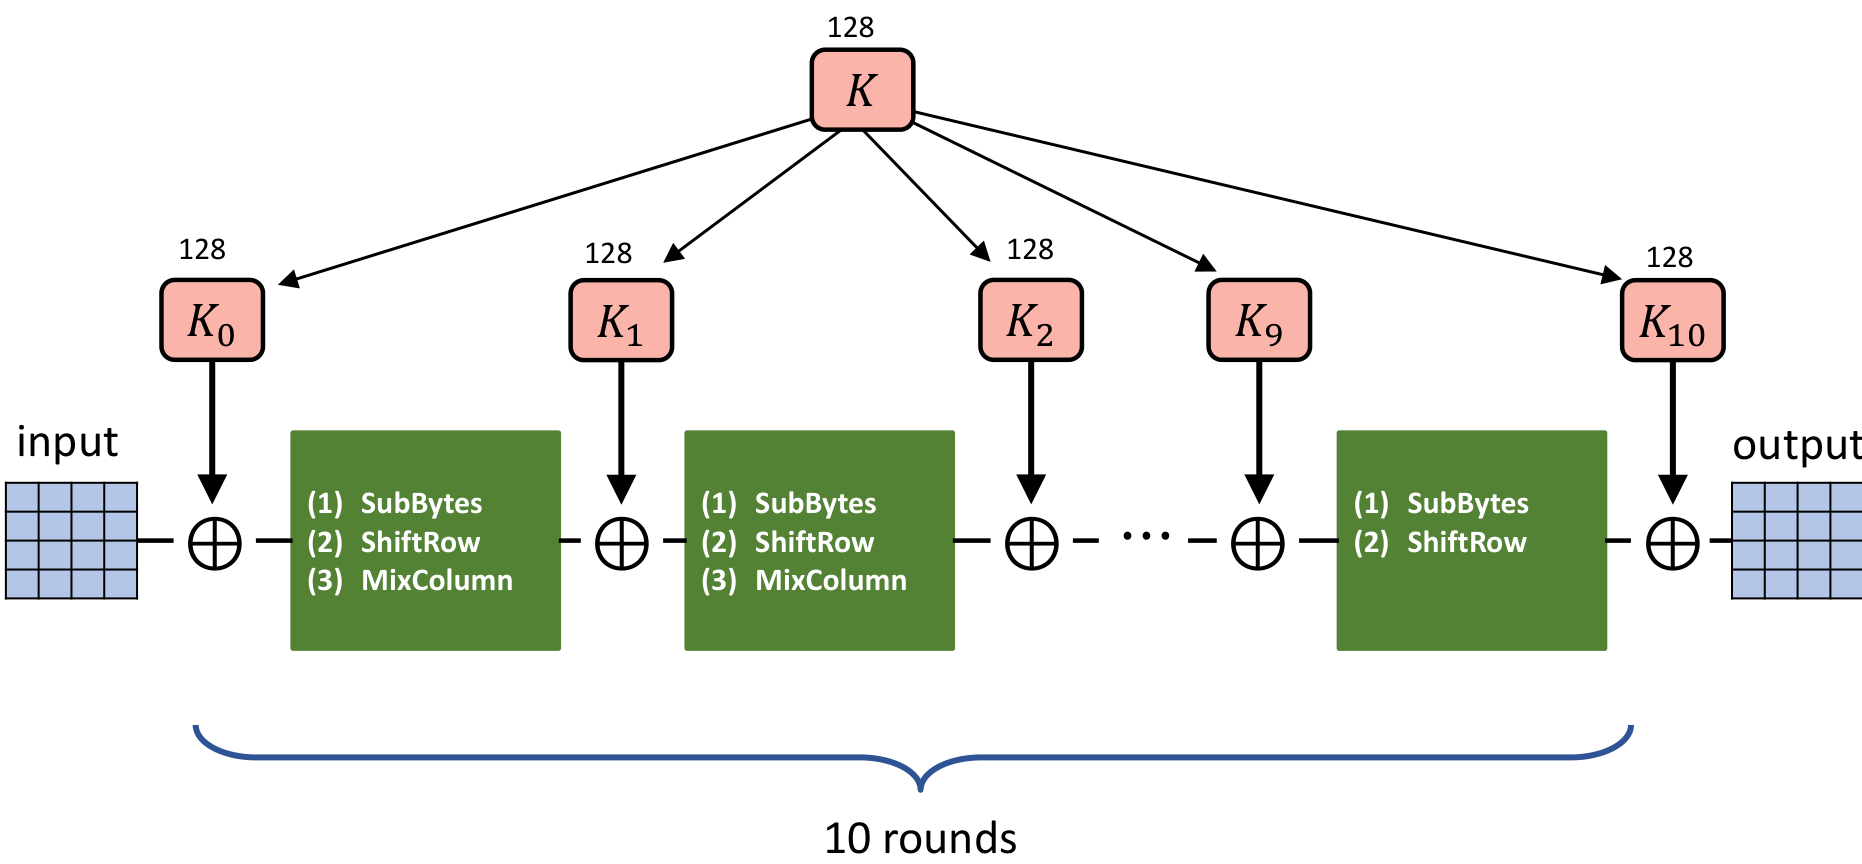
\includegraphics[width=0.85\linewidth, height=0.82\textheight, keepaspectratio]{figures/alur-enkripsi-aes.png}
    \caption{Alur enkripsi AES-128: kunci diekspansi menjadi \textit{round key}, dan \textit{state} diproses melalui SubBytes, ShiftRows, serta MixColumns selama 10 putaran}
    \label{fig:alur-enkripsi-aes}
    \sumber{Munir, \textit{IF4020 Kriptografi}, ITB.}
\end{figure}

% Ilustrasi SubBytes: satu byte matriks state dipetakan melalui S-box menjadi
% byte baru. Digambar ulang sebagai diagram vektor; penggambaran aslinya dari
% slide Munir ditangkap pada bingkai animasi yang sorotannya meleset sehingga
% kotak sorot menutupi sel tetangga dan panahnya menunjuk baris yang salah.
% Dirujuk dari section-02.tex dengan % Ilustrasi SubBytes: satu byte matriks state dipetakan melalui S-box menjadi
% byte baru. Digambar ulang sebagai diagram vektor; penggambaran aslinya dari
% slide Munir ditangkap pada bingkai animasi yang sorotannya meleset sehingga
% kotak sorot menutupi sel tetangga dan panahnya menunjuk baris yang salah.
% Dirujuk dari section-02.tex dengan % Ilustrasi SubBytes: satu byte matriks state dipetakan melalui S-box menjadi
% byte baru. Digambar ulang sebagai diagram vektor; penggambaran aslinya dari
% slide Munir ditangkap pada bingkai animasi yang sorotannya meleset sehingga
% kotak sorot menutupi sel tetangga dan panahnya menunjuk baris yang salah.
% Dirujuk dari section-02.tex dengan \input{figures/subbytes-aes}.
\begin{figure}[htbp]
    \centering
    \begin{tikzpicture}[
        sel/.style={draw, minimum size=1.15cm, inner sep=0pt, font=\small},
        sorot/.style={sel, fill=blue!55, text=white},
        panah/.style={-{Latex[length=2.4mm]}, thick},
    ]
        % Grid state (kiri) dan state' (kanan). Indeks mengikuti penamaan slide:
        % baris pertama a_00..a_03, dan seterusnya.
        \foreach \i in {0,1,2,3} {
            \foreach \j in {0,1,2,3} {
                \node[sel] (a\i\j) at ({\j*1.15}, {-\i*1.15}) {$a_{\i\j}$};
                \node[sel] (b\i\j) at ({\j*1.15+8.05}, {-\i*1.15}) {$b_{\i\j}$};
            }
        }
        % Byte yang sedang disubstitusi ditandai. Dipilih byte pada baris
        % terakhir agar panahnya dapat keluar tepat di tepi bawah grid tanpa
        % melintasi sel atau label lain.
        \node[sorot] at (a31) {$a_{31}$};
        \node[sorot] at (b31) {$b_{31}$};

        \node[font=\small] at (1.725, 1.15) {state};
        \node[font=\small] at (9.775, 1.15) {state$'$};

        \node[draw, thick, fill=white, minimum width=1.9cm, minimum height=1.1cm,
              font=\small] (sbox) at (5.75,-5.3) {S-box};

        % Byte tersorot masuk ke S-box, lalu keluar sebagai byte hasil substitusi.
        \draw[panah] (a31.south) to[out=-90, in=175] (sbox.west);
        \draw[panah] (sbox.east) to[out=5, in=-90] (b31.south);
    \end{tikzpicture}
    \caption{Transformasi SubBytes pada AES: setiap byte matriks \textit{state} disubstitusi melalui tabel S-box menjadi byte baru}
    \label{fig:subbytes-aes}
    \sumber{Munir, \textit{IF4020 Kriptografi}, ITB.}
\end{figure}
.
\begin{figure}[htbp]
    \centering
    \begin{tikzpicture}[
        sel/.style={draw, minimum size=1.15cm, inner sep=0pt, font=\small},
        sorot/.style={sel, fill=blue!55, text=white},
        panah/.style={-{Latex[length=2.4mm]}, thick},
    ]
        % Grid state (kiri) dan state' (kanan). Indeks mengikuti penamaan slide:
        % baris pertama a_00..a_03, dan seterusnya.
        \foreach \i in {0,1,2,3} {
            \foreach \j in {0,1,2,3} {
                \node[sel] (a\i\j) at ({\j*1.15}, {-\i*1.15}) {$a_{\i\j}$};
                \node[sel] (b\i\j) at ({\j*1.15+8.05}, {-\i*1.15}) {$b_{\i\j}$};
            }
        }
        % Byte yang sedang disubstitusi ditandai. Dipilih byte pada baris
        % terakhir agar panahnya dapat keluar tepat di tepi bawah grid tanpa
        % melintasi sel atau label lain.
        \node[sorot] at (a31) {$a_{31}$};
        \node[sorot] at (b31) {$b_{31}$};

        \node[font=\small] at (1.725, 1.15) {state};
        \node[font=\small] at (9.775, 1.15) {state$'$};

        \node[draw, thick, fill=white, minimum width=1.9cm, minimum height=1.1cm,
              font=\small] (sbox) at (5.75,-5.3) {S-box};

        % Byte tersorot masuk ke S-box, lalu keluar sebagai byte hasil substitusi.
        \draw[panah] (a31.south) to[out=-90, in=175] (sbox.west);
        \draw[panah] (sbox.east) to[out=5, in=-90] (b31.south);
    \end{tikzpicture}
    \caption{Transformasi SubBytes pada AES: setiap byte matriks \textit{state} disubstitusi melalui tabel S-box menjadi byte baru}
    \label{fig:subbytes-aes}
    \sumber{Munir, \textit{IF4020 Kriptografi}, ITB.}
\end{figure}
.
\begin{figure}[htbp]
    \centering
    \begin{tikzpicture}[
        sel/.style={draw, minimum size=1.15cm, inner sep=0pt, font=\small},
        sorot/.style={sel, fill=blue!55, text=white},
        panah/.style={-{Latex[length=2.4mm]}, thick},
    ]
        % Grid state (kiri) dan state' (kanan). Indeks mengikuti penamaan slide:
        % baris pertama a_00..a_03, dan seterusnya.
        \foreach \i in {0,1,2,3} {
            \foreach \j in {0,1,2,3} {
                \node[sel] (a\i\j) at ({\j*1.15}, {-\i*1.15}) {$a_{\i\j}$};
                \node[sel] (b\i\j) at ({\j*1.15+8.05}, {-\i*1.15}) {$b_{\i\j}$};
            }
        }
        % Byte yang sedang disubstitusi ditandai. Dipilih byte pada baris
        % terakhir agar panahnya dapat keluar tepat di tepi bawah grid tanpa
        % melintasi sel atau label lain.
        \node[sorot] at (a31) {$a_{31}$};
        \node[sorot] at (b31) {$b_{31}$};

        \node[font=\small] at (1.725, 1.15) {state};
        \node[font=\small] at (9.775, 1.15) {state$'$};

        \node[draw, thick, fill=white, minimum width=1.9cm, minimum height=1.1cm,
              font=\small] (sbox) at (5.75,-5.3) {S-box};

        % Byte tersorot masuk ke S-box, lalu keluar sebagai byte hasil substitusi.
        \draw[panah] (a31.south) to[out=-90, in=175] (sbox.west);
        \draw[panah] (sbox.east) to[out=5, in=-90] (b31.south);
    \end{tikzpicture}
    \caption{Transformasi SubBytes pada AES: setiap byte matriks \textit{state} disubstitusi melalui tabel S-box menjadi byte baru}
    \label{fig:subbytes-aes}
    \sumber{Munir, \textit{IF4020 Kriptografi}, ITB.}
\end{figure}


\begin{figure}[htbp]
    \centering
    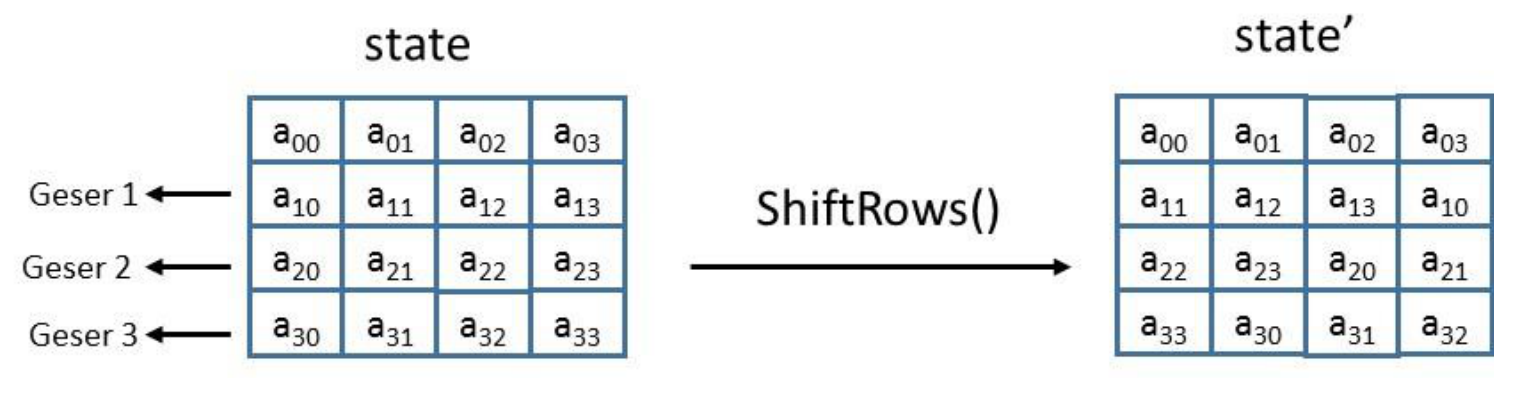
\includegraphics[width=0.95\linewidth, height=0.82\textheight, keepaspectratio]{figures/shiftrows-aes.png}
    \caption{Transformasi ShiftRows pada AES: baris ke-$r$ matriks \textit{state} digeser secara siklik ke kiri sejauh $r$ byte}
    \label{fig:shiftrows-aes}
    \sumber{Munir, \textit{IF4020 Kriptografi}, ITB.}
\end{figure}
